\documentclass{article}

\usepackage{graphicx}
\usepackage{tikz}
\usepackage{tikzsymbols}
\usetikzlibrary{calc,patterns,shapes.geometric}
\pagestyle{empty}
\usepackage[margin=0pt]{geometry}
\geometry{papersize={14in,12in}}

\def\centerarc[#1](#2)(#3:#4:#5){\draw[#1] ($(#2)+({#5*cos(#3)},{#5*sin(#3)})$) arc (#3:#4:#5);}

\begin{document}
	\begin{figure}
		\centering
		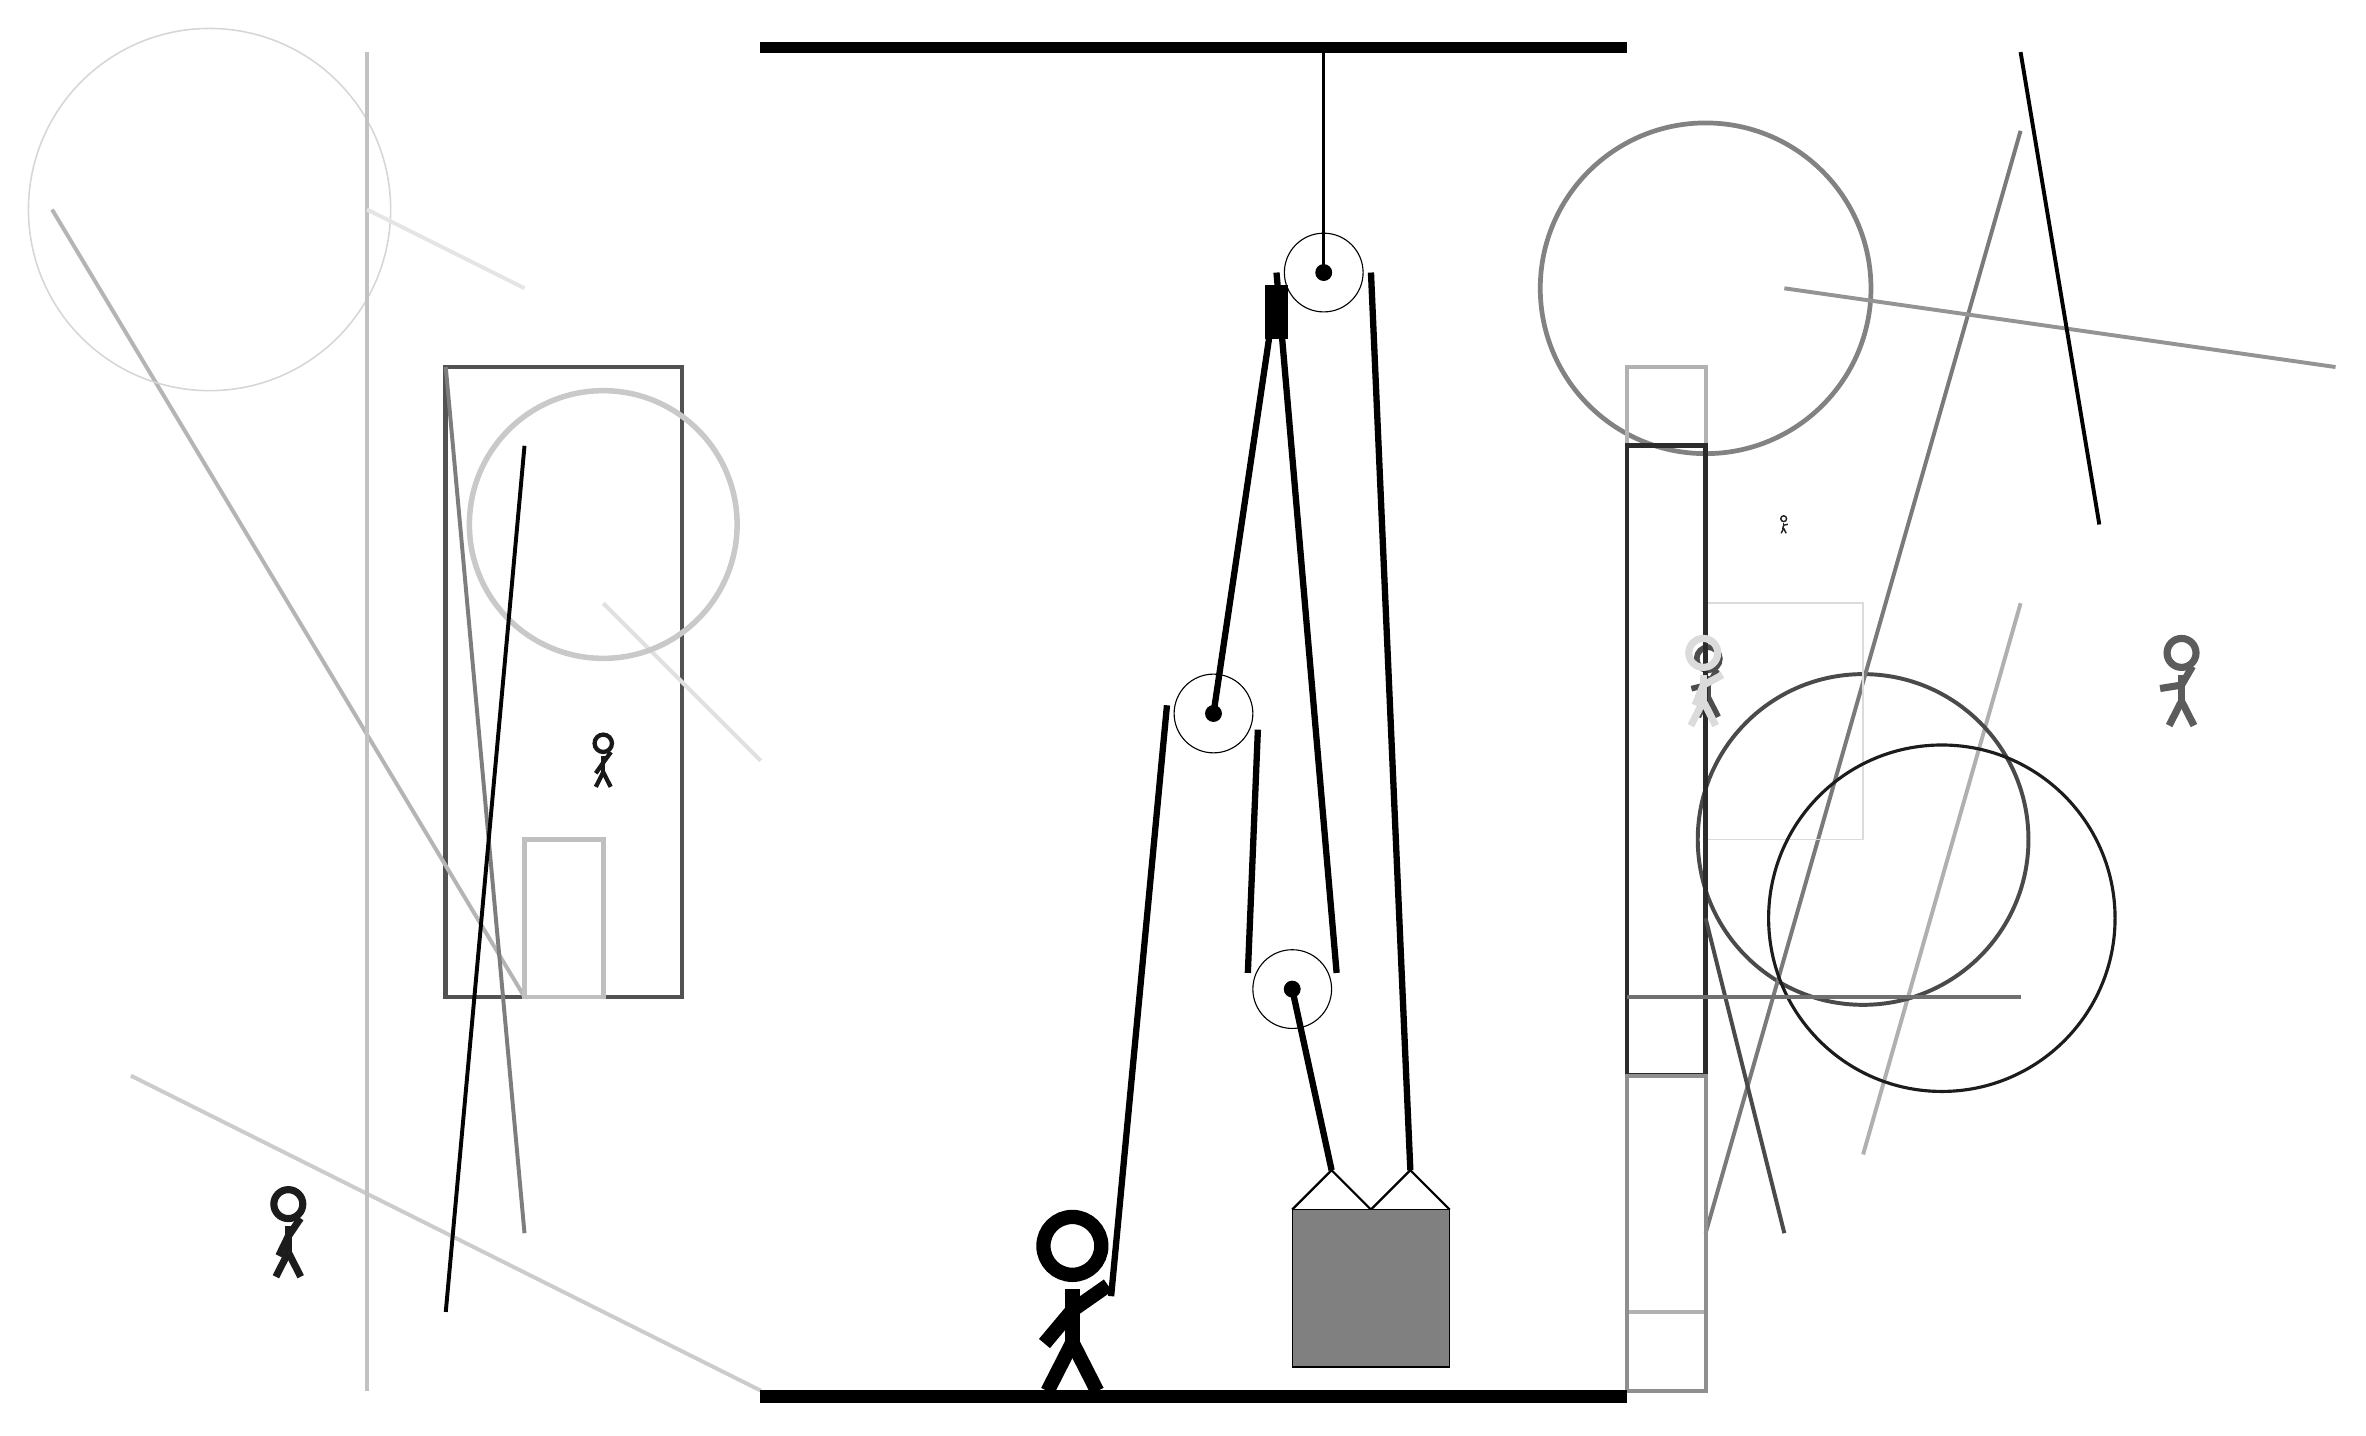
\begin{tikzpicture}
			%%%%% START %%%%%
			
			\draw[fill=black] (-6, 14) rectangle (5, 14.125);
			
			\draw (-0.25, 5.6) circle (0.5);
			\draw[fill=black] (-0.25, 5.6) circle (0.1);
			
			\draw (0.75, 2.1) circle (0.5);
			\draw[fill=black] (0.75, 2.1) circle (0.1);
			
			\draw [line width=0.6mm, color=black!49](6, 11) circle (2.1);
			
			\draw[line width=0.6mm, color=black!68] (-7, 2) rectangle (-10, 10);
			\draw[line width=0.5mm, color=black!31](10, 7) -- (8, 0);
			\draw [line width=0.5mm, color=black!71](8, 4) circle (2.1);
			\draw[line width=0.5mm, color=black!29](-9, 2) -- (-15, 12);
			
			\draw[line width=0.5mm, color=black!52](6, -1) -- (10, 13);
			\draw[line width=0.5mm, color=black!20](-6, -3) -- (-14, 1);
			
			\draw [line width=0.2mm, color=black!16](-13, 12) circle (2.3);
			\draw[line width=0.2mm, color=black!14] (6, 7) rectangle (8, 4);
			
			\node[line width=0.4mm, color=black!70] at (6, 6) {\Strichmaxerl[4][14][59]};
			\node[line width=0.4mm, color=black!87] at (7, 8) {\Strichmaxerl[1][76][11]};
			\draw[line width=0.5mm, color=black!12](-8, 7) -- (-6, 5);
			\draw[line width=0.5mm, color=black!30] (6, 10) rectangle (5, -2);
			
			\node[line width=0.4mm, color=black!64] at (12, 6) {\Strichmaxerl[5][9][60]};
			\draw[line width=0.5mm, color=black!51](-9, -1) -- (-10, 10);
			\draw[line width=0.5mm, color=black!24](-11, -3) -- (-11, 14);
			
			\draw[line width=0.5mm, color=black!10](-11, 12) -- (-9, 11);
			
			\draw[line width=0.5mm, color=black!42](7, 11) -- (14, 10);
			\draw[line width=0.6mm, color=black!83] (5, 9) rectangle (6, 1);
			\node[line width=0.3mm, color=black!14] at (6, 6) {\Strichmaxerl[5][68][28]};
			\draw[line width=0.5mm, color=black!100](10, 14) -- (11, 8);
			
			\draw [line width=0.4mm, color=black!89](9, 3) circle (2.2);
			\draw[line width=0.5mm, color=black!44] (5, -3) rectangle (6, 1);
			\node[line width=0.5mm, color=black!89] at (-12, -1) {\Strichmaxerl[5][64][56]};
			\draw [line width=0.7mm, color=black!21](-8, 8) circle (1.7);
			\draw[line width=0.6mm, color=black!25] (-8, 2) rectangle (-9, 4);
			
			\node[line width=0.2mm, color=black!90] at (-8, 5) {\Strichmaxerl[3][55][54]};
			\draw[line width=0.5mm, color=black!99](-9, 9) -- (-10, -2);
			\draw[line width=0.5mm, color=black!71](7, -1) -- (6, 3);
			
			\draw[line width=0.5mm, color=black!56](10, 2) -- (5, 2);
			
			\draw (1.15, 11.2) circle (0.5);
			\draw[fill=black] (1.15, 11.2) circle (0.1);
			\draw[very thick] (1.15, 11.2) -- (1.15, 14);
			
			\draw[thick]  (0.75, -0.7) -- (1.25, -0.2) -- (1.75, -0.7) -- (2.25, -0.2) -- (2.75, -0.7);
			\draw[fill=black!50] (0.75, -0.7) rectangle (2.75, -2.7);
			
			\draw[line width=0.8mm] (-0.25, 5.6) -- (0.55, 11.0);
			\draw[line width=0.8mm, fill=black](0.45, 10.4) rectangle (0.65, 11.0);
			\draw[line width=0.8mm] (-1.55, -1.8) -- (-0.8409, 5.7042);
			\centerarc[line width=0.8mm](-0.25, 5.6)(-20:170:0.6);
			\draw[line width=0.8mm] (0.3138, 5.3948) -- (0.1862, 2.3052);
			\centerarc[line width=0.8mm](0.75, 2.1)(160:380:0.6);
			\draw[line width=0.8mm] (1.3138, 2.3052) -- (0.55, 11.2);
			\draw[line width=0.8mm](0.75, 2.1) -- (1.25, -0.2);
			\centerarc[line width=0.8mm](1.15, 11.2)(0:180:0.6);
			\draw[line width=0.8mm] (1.75, 11.2) -- (2.25, -0.2);
			
			\node at (-2, -1.9) {\Strichmaxerl[10][50][35]};
			
			\draw[fill=black] (-6, -3) rectangle (5, -3.15);
			
			%%%%% END %%%%%
		\end{tikzpicture}
	\end{figure}	
\end{document}